\documentclass[11pt, oneside]{article}   	% use "amsart" instead of "article" for AMSLaTeX format
\usepackage{geometry}                		% See geometry.pdf to learn the layout options. There are lots.
\geometry{letterpaper}                   		% ... or a4paper or a5paper or ... 
%\geometry{landscape}                		% Activate for for rotated page geometry
%\usepackage[parfill]{parskip}    		% Activate to begin paragraphs with an empty line rather than an indent
\usepackage{graphicx}				% Use pdf, png, jpg, or eps§ with pdflatex; use eps in DVI mode
								% TeX will automatically convert eps --> pdf in pdflatex		
\usepackage{amssymb}
\usepackage{amsmath}
\usepackage{parskip}
\usepackage{color}
\usepackage{hyperref}

\title{The End}
%\author{The Author}
%\section{}
%\subsection*{}
\date{}							% Activate to display a given date or no date

\graphicspath{{/Users/telliott_admin/Dropbox/Tex/png/}}
% \begin{center} 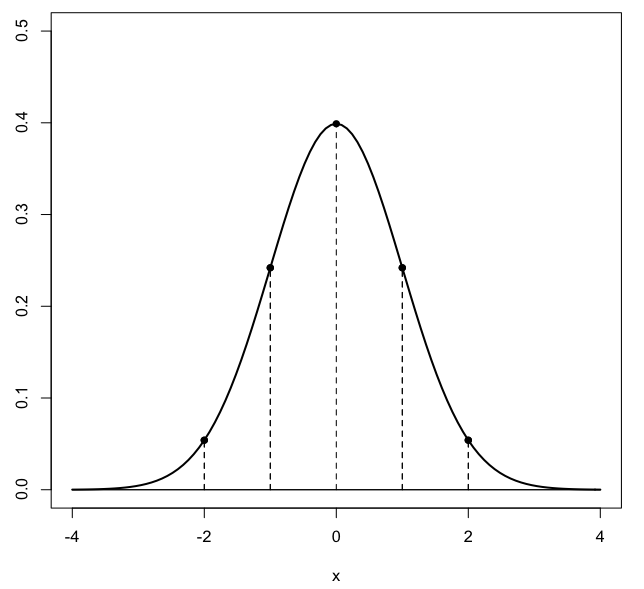
\includegraphics [scale=0.4] {gauss3.png} \end{center}
\begin{document}
\maketitle
\Large
So now, let's go back to the integrals we listed at the very beginning:
\[ \int_0^{\infty} \frac{\sin^2 x}{x^2} \ dx = \frac{\pi}{2} \]
\[ \int_0^{\infty} \frac{x^{\alpha - 1}}{1 + x} \ dx = \frac{\pi}{\sin \alpha \pi} \]
\[ \int_0^{2 \pi} \frac{1}{a + \sin \theta} \ d \theta = \frac{2 \pi}{\sqrt{a^2 - 1}} \]

Can we solve these now?  
\subsection*{problem 1}
We solved a problem related to the first integral previously:
\[ \int_0^{\infty} \frac{\sin x}{x} \ dx = \frac{\pi}{2} \]
How to make use of that?

Start with the sum of angles:
\[ \cos (s+t) = \cos s \cos t - \sin s \sin t \]
\[ \cos (s-t) = \cos s \cos (-t) - \sin s \sin (-t) \]
\[ = \cos s \cos t + \sin s \sin t \]
Adding the minus the first to the second gives:
\[ \cos (s-t) - \cos(s+t) = 2 \sin s \sin t \]
For the general problem, we obtain
\[ 2 \ \frac{\sin(ax) \sin(bx)}{x^2} =  \frac{\cos ((a-b)x) - \cos((a+b)x) }{x^2}  \]

Now if we consider a function of $y$
\[ \frac{\sin x y}{x} \ dy \]
the integral of this function is
\[ \int \frac{\sin x y}{x} \ dy = -\frac{1}{x^2} \ [ \cos x y \ ] + C \]
Suppose we use as bounds $a-b$ and $a+b$
\[ \int_{a-b}^{a+b} \frac{\sin x y}{x} \ dy = -\frac{1}{x^2} \ [ \cos (a+b) x  - \cos(a-b) x \ ] \]
\[  \int_{a-b}^{a+b} \frac{\sin x y}{x} \ dy = \frac{1}{x^2} \ [ \cos (a-b) x  + \cos(a+b) x \ ] \]

Hence, going back to our problem
\[ 2 \ \frac{\sin(ax) \sin(bx)}{x^2} =  \frac{\cos ((a-b)x) - \cos((a+b)x) }{x^2}  \]
and integrating both sides we see that
\[ 2 \int_0^{\infty} \frac{\sin ax \sin bx}{x^2} \ dx = \int_0^{\infty} \int_{a-b}^{a+b} \frac{\sin x y}{x} \ dy  \ dx \]
Change the order of integration:
\[ = \int_{a-b}^{a+b} \int_0^{\infty} \frac{\sin x y}{x} \ dx  \ dy \]

for the inner integral $y$ is constant.  Substitute $t = xy$, so $1/x = y/t$ and $dt = y \ dx$ and we have
\[ \int_0^{\infty} \frac{\sin x y}{x} \ dx = y \frac{\sin t}{t} \ \frac{1}{y} \ dt \]
\[ = \int_0^{\infty}  \frac{\sin t}{t} \ \ dt = \frac{\pi}{2} \]
so the outer integral is
\[ \frac{\pi}{2} \int_{a-b}^{a+b}  \ dy = \frac{\pi}{2} \ 2b = \pi b \]
In this problem, $a = b = 1$ so
\[ 2 \int_0^{\infty} \frac{\sin^2 x}{x^2} \ dx = \pi \]
\[ \int_0^{\infty} \frac{\sin^2 x}{x^2} \ dx = \frac{\pi}{2} \]
That was a little harder than I expected!  Notice the result that
\[ \int_0^{\infty} \frac{\sin^2 x}{x^2} \ dx = \int_0^{\infty} \frac{\sin x}{x} \ dx  \]

\subsection*{problem 2}
\[ \int_0^{\infty} \frac{x^{\alpha - 1}}{1 + x} \ dx = \frac{\pi}{\sin \alpha \pi} \]
Write the complex integral
\[ \int \frac{z^{\alpha - 1}}{1 + z} \ dz \]
This has a simple pole at $z = -1$, so any integral that includes that pole will have the value
\[ \text{Res }(-1) = (-1)^{\alpha - 1} \]
But we want the base of our contour to include $0 \rightarrow \infty$ (we don't need to include the pole), hence
\[ \oint f(z) \ dz = 0 \]
\[ = \int_0^{\infty} \frac{x^{\alpha - 1}}{1 + x} \ dx + \int_0^{\pi/2} \frac{z^{\alpha - 1}}{1 + z} \ dz \]
say that
\[ z = Re^{i \theta} \]
\[ dz = i z \ d \theta \]

??

\subsection*{problem 3}
\[ \int_0^{2 \pi} \frac{1}{a + \sin \theta} \ d \theta = \frac{2 \pi}{\sqrt{a^2 - 1}} \]

Previously we solved a similar problem
\[ \int_0^{2\pi} \frac{1}{2 + \cos \theta} \ d \theta \]

Recall there that we said that the equation for an ellipse in polar coordinates (with one focus at the origin) is
\[ r = \frac{b^2}{a - c \cos \theta} \]

Neglect the minus sign (which just flips the orientation along the $x$-axis) and write
\[ r = \frac{b^2}{a + c \cos \theta} \]

Let $a=2$ and $c=1$ and
\[ b^2 = a^2 - c^2 = 3 \]

Substituting
\[ r = \frac{3}{2 + \cos \theta} \]
\[ 3 r = \frac{1}{2 + \cos \theta} \]

What the integral seems to be is the integral of $r \ d \theta$ around an ellipse with $a = 2$ and $b = \sqrt{3}$.  This would be $r d \theta$ added up over the perimeter of that ellipse, i.e. the area.  

The area would be $\pi a b = \pi 2 \sqrt{3}$.  $3$ times the value of the integral is equal to this so
\[ I = \frac{1}{3} \ \pi 2 \sqrt{3} =  \pi \frac{2}{\sqrt{3}} \]

Substitution of $\sin \theta$ for $\cos \theta$ just rotates the ellipse.

Let's solve the given problem:
\[ \int_0^{2 \pi} \frac{1}{a + \sin \theta} \ d \theta \]

write
\[ e^{i \theta} = \cos \theta + i \sin \theta \]
\[ e^{-i \theta} = \cos \theta - i \sin \theta \]
Subtract
\[ e^{i \theta} - e^{-i \theta} = 2i \sin \theta \]
\[ \sin \theta = \frac{1}{2i} \ (e^{i \theta} - e^{-i \theta}) \]

Suppose our contour is the unit disk centered at zero.  Then
\[ \frac{1}{a + \sin \theta} = \frac{1}{a + 1/2i (z + 1/z)} \]
and
\[ dz = iz \ d \theta \]
as we've seen before, so we have
\[  \int_0^{2 \pi} \frac{1}{a + \sin \theta} \ d \theta = \oint \frac{1}{a + 1/2i (z + 1/z)} \ \frac{1}{iz} \ dz \]
\[ = \oint \frac{1}{iaz - 1/2 (z^2 + 1)} \ \ dz \]




\end{document}  